\section{Results}
\label{sec:results}

\subsection{Main Results}
\label{sec:main_results}

\Tabref{tab:main} presents the main results averaged over five random seeds. Both the joint and specialized models achieve remarkably low calibration error, but they differ substantially in accuracy.

\begin{table}[t]
    \centering
    \caption{Main results (mean $\pm$ std over 5 seeds). Both models achieve low ECE, but the specialized model has substantially better accuracy (F1) and Brier score. Best results in \textbf{bold}; differences in ECE are not statistically significant ($p = 0.27$).}
    \begin{tabular}{@{}lcccc@{}}
        \toprule
        \textbf{Model} & \textbf{ECE} $\downarrow$ & \textbf{Brier} $\downarrow$ & \textbf{Accuracy} $\uparrow$ & \textbf{F1} $\uparrow$ \\
        \midrule
        \joint           & \textbf{0.0065} {\scriptsize $\pm$ 0.0017} & 0.0239 {\scriptsize $\pm$ 0.0021} & 0.970 {\scriptsize $\pm$ 0.004} & 0.969 {\scriptsize $\pm$ 0.004} \\
        \specialized     & 0.0078 {\scriptsize $\pm$ 0.0012} & \textbf{0.0128} {\scriptsize $\pm$ 0.0012} & \textbf{0.986} {\scriptsize $\pm$ 0.001} & \textbf{0.985} {\scriptsize $\pm$ 0.001} \\
        \tempscaled      & \textbf{0.0063} {\scriptsize $\pm$ 0.0021} & 0.0238 {\scriptsize $\pm$ 0.0020} & 0.970 {\scriptsize $\pm$ 0.004} & 0.969 {\scriptsize $\pm$ 0.004} \\
        \bottomrule
    \end{tabular}
    \label{tab:main}
\end{table}

\para{Calibration.} The joint model achieves ECE of 0.0065 and the specialized model achieves 0.0078---both well below the 0.05 threshold typically considered ``well-calibrated.'' A paired $t$-test finds no significant difference ($t = -1.27$, $p = 0.27$), with a medium effect size (Cohen's $d = -0.64$). Temperature scaling marginally improves the joint model's ECE to 0.0063, with optimal temperatures consistently near 1.0 (range: 1.03--1.11), confirming both models are already well-calibrated.

\para{Accuracy.} The specialized model substantially outperforms the joint model in copy decision accuracy: F1 of 0.985 versus 0.969, representing a 52\% reduction in error rate. This gap is consistent across all five seeds, with the specialized model's variance also notably lower (std = 0.001 vs.\ 0.004).

\para{Brier score.} The Brier score favors the specialized model by 46\% (0.0128 vs.\ 0.0239). Since both models have similar calibration, this improvement comes almost entirely from better \emph{refinement}---the specialized model produces more confident predictions that are also more often correct.

\para{Worst-case calibration.} \Tabref{tab:mce} shows the maximum calibration error. The specialized model has lower MCE (0.214 vs.\ 0.332) and substantially lower variance (std = 0.068 vs.\ 0.173), indicating more consistent calibration across the probability range.

\begin{table}[t]
    \centering
    \caption{Maximum calibration error (MCE) over 5 seeds. The specialized model has lower and more stable worst-case calibration.}
    \begin{tabular}{@{}lc@{}}
        \toprule
        \textbf{Model} & \textbf{MCE} $\downarrow$ \\
        \midrule
        \joint       & 0.332 {\scriptsize $\pm$ 0.173} \\
        \specialized & \textbf{0.214} {\scriptsize $\pm$ 0.068} \\
        \tempscaled  & 0.311 {\scriptsize $\pm$ 0.129} \\
        \bottomrule
    \end{tabular}
    \label{tab:mce}
\end{table}

\subsection{Reliability Diagrams}
\label{sec:reliability}

\Figref{fig:reliability} shows the reliability diagrams for both models. Both track the diagonal closely, consistent with the low ECE values. The joint model shows slightly more deviation in a few bins, consistent with its higher MCE.

\begin{figure}[t]
    \centering
    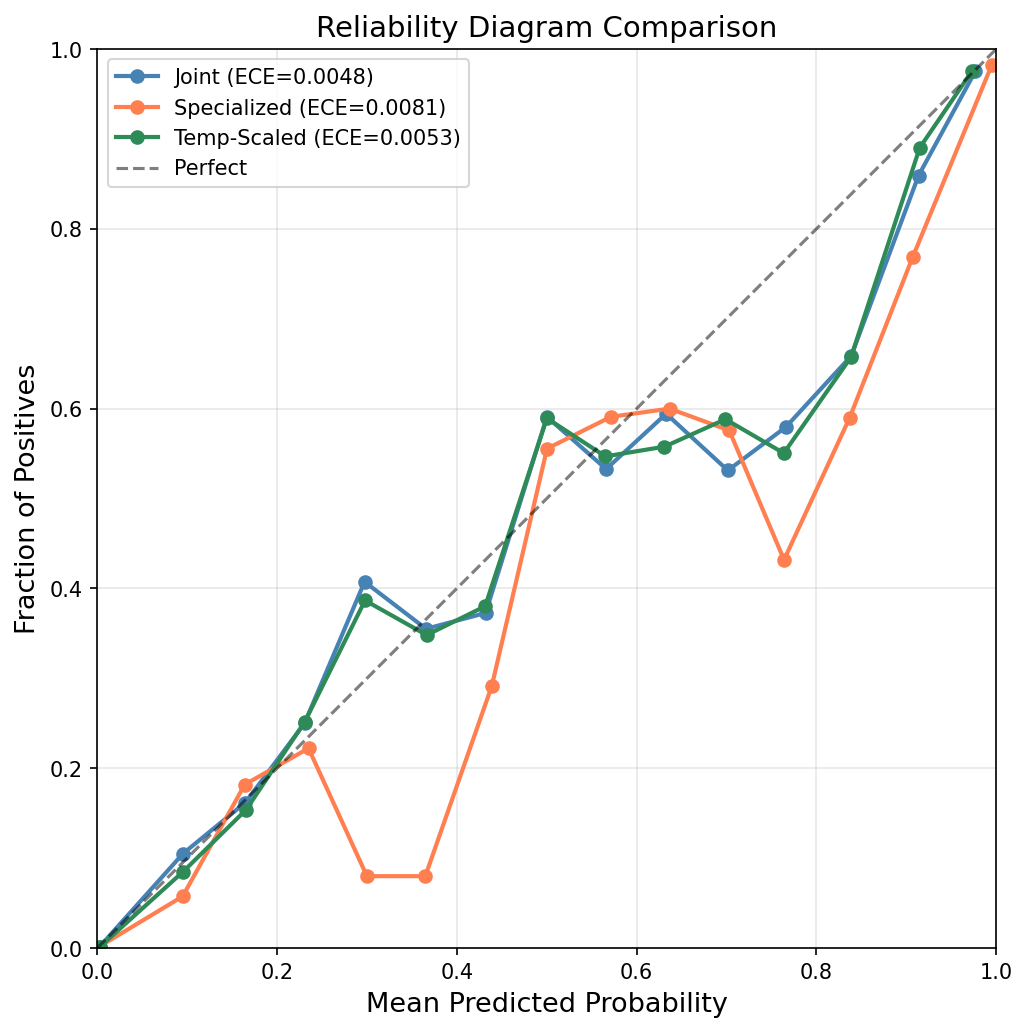
\includegraphics[width=0.95\linewidth]{figures/combined_reliability.png}
    \caption{Reliability diagrams comparing the joint pointer-generator and specialized copy-decider. Both models closely track the diagonal (perfect calibration). The joint model shows occasional deviations in individual bins, consistent with its higher MCE.}
    \label{fig:reliability}
\end{figure}

\subsection{Model Size Ablation}
\label{sec:ablation}

We ablate model size to test whether the calibration relationship holds across scales. \Tabref{tab:ablation} shows results for three configurations (single seed).

\begin{table}[t]
    \centering
    \caption{Model size ablation (seed = 42). The specialized model consistently outperforms in F1 across all sizes. Calibration shows an interaction: the joint model improves more with scale.}
    \begin{tabular}{@{}lccccc@{}}
        \toprule
        & \multicolumn{2}{c}{\textbf{ECE} $\downarrow$} & \multicolumn{2}{c}{\textbf{F1} $\uparrow$} & \\
        \cmidrule(lr){2-3} \cmidrule(lr){4-5}
        \textbf{Size} & \textbf{Joint} & \textbf{Spec.} & \textbf{Joint} & \textbf{Spec.} & \textbf{Params (J / S)} \\
        \midrule
        Tiny (1L, $d$=64)   & 0.0192 & \textbf{0.0179} & 0.918 & \textbf{0.968} & 157K / 69K \\
        Small (2L, $d$=128)  & 0.0106 & \textbf{0.0100} & 0.957 & \textbf{0.982} & 824K / 472K \\
        Medium (4L, $d$=256) & \textbf{0.0053} & 0.0092 & 0.979 & \textbf{0.983} & 5.7M / 3.5M \\
        \bottomrule
    \end{tabular}
    \label{tab:ablation}
\end{table}

\para{Accuracy scales consistently.} The specialized model achieves higher F1 at every size, with the largest advantage at the tiny scale (0.968 vs.\ 0.918, a 61\% error reduction). The gap narrows at medium scale (0.983 vs.\ 0.979) but remains in favor of specialization.

\para{Calibration shows an interaction.} At tiny and small scales, the specialized model has slightly better ECE. At medium scale, the joint model achieves notably better ECE (0.0053 vs.\ 0.0092). This suggests that as model capacity increases, the joint model's generation loss provides increasing calibration regularization, while the specialized model may slightly overfit to the copy decision.

\begin{figure}[t]
    \centering
    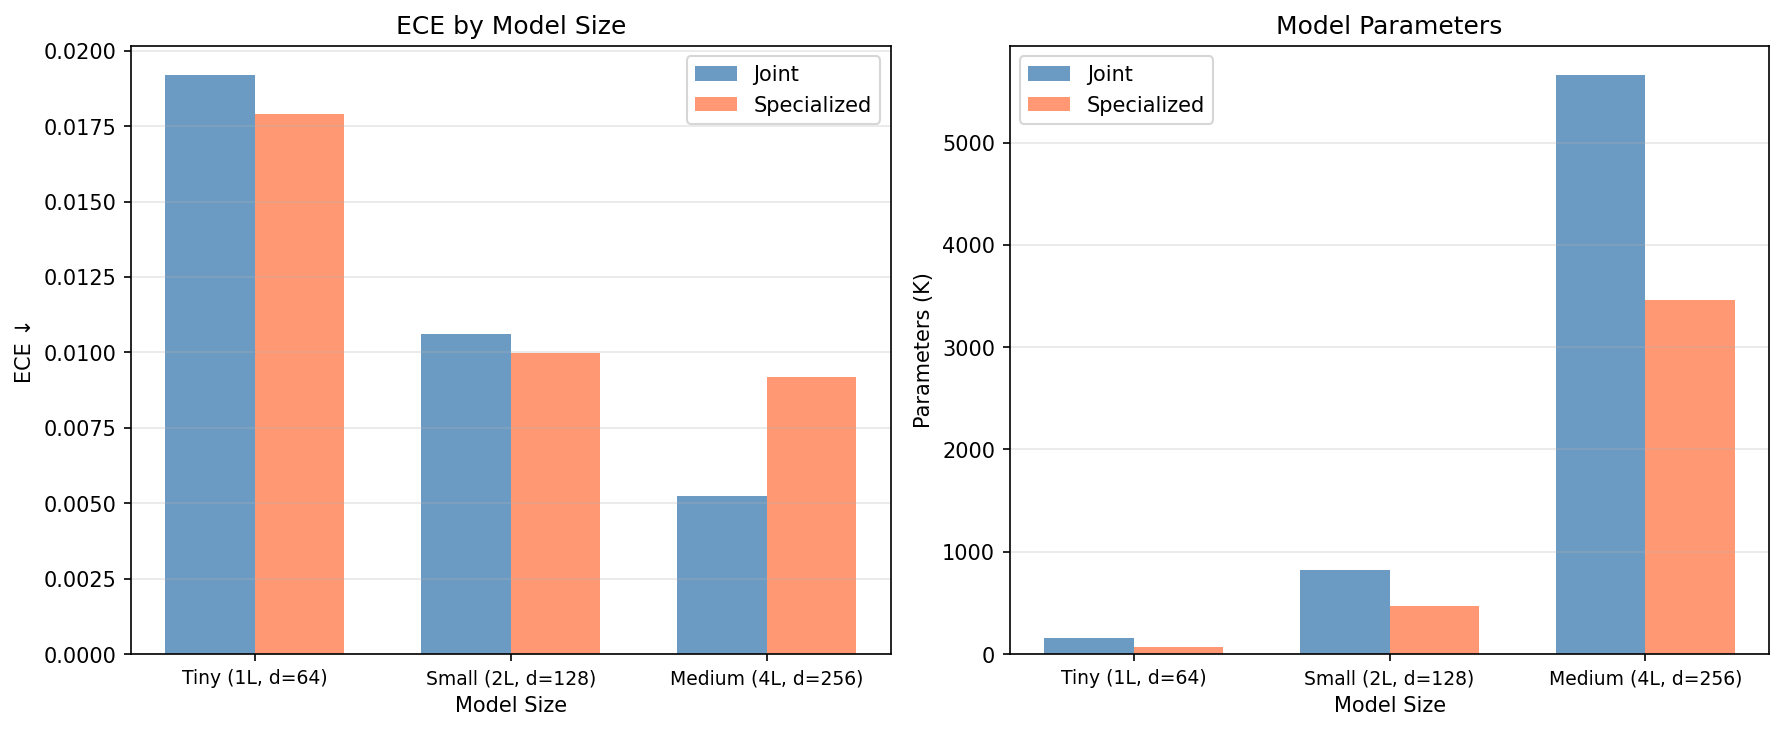
\includegraphics[width=0.95\linewidth]{figures/size_ablation.png}
    \caption{Model size ablation showing ECE and F1 across three scales. The specialized model consistently achieves higher F1, while the joint model's ECE improves more rapidly with scale, surpassing the specialized model at medium size.}
    \label{fig:ablation}
\end{figure}

\subsection{Statistical Analysis}
\label{sec:stats}

\Tabref{tab:stats} summarizes the statistical tests. The ECE difference between the joint and specialized models is not significant at $\alpha = 0.05$, nor is the difference between the temperature-scaled and specialized models. The medium Cohen's $d$ suggests a meaningful trend that may reach significance with more seeds or larger test sets.

\begin{table}[t]
    \centering
    \caption{Statistical tests for ECE comparisons. No comparison reaches significance at $\alpha = 0.05$.}
    \begin{tabular}{@{}lccc@{}}
        \toprule
        \textbf{Comparison} & \textbf{$t$-stat} & \textbf{$p$-value} & \textbf{Cohen's $d$} \\
        \midrule
        Joint vs.\ Specialized       & $-1.27$ & 0.272 & $-0.64$ \\
        TempScaled vs.\ Specialized   & $-1.01$ & 0.371 & --- \\
        \bottomrule
    \end{tabular}
    \label{tab:stats}
\end{table}